\listfiles
\documentclass[a4paper, twocolumn]{article}

\usepackage{polski}
\usepackage[utf8]{inputenc}
\usepackage[twoside=true, left=25mm, right=25mm, top=25mm, bottom=25mm,paper=a4paper]{geometry}
\usepackage{graphicx}

\title{Biotechnologia}
\author{domka i janek}
\begin{document}
\maketitle
\section{Czym jest biotechnologia?}%
\label{sec:Czym jest biotechnologia?}
\textbf{Biotechnologia} - dyscyplina naukowa, która zajmuje się wykorzystywaniem organizmów, wirusów lub ich składników do celów praktycznych.
\section{Czym zajmuje się biotechnologia tradycyjna i molekularna?}%
\label{sec:Czym zajmuje się biotechnologia tradycyjna i molekularna?}
\textbf{Biotechnologia tradycyjna} (\textit{klasyczna}) - wykorzystuje naturalnie występujące w przyrodzie wirusy, organizmy lub produkowane przez nie substancje.
Dobór organizmów o pożądanych cechach odbywa się przez selekcje sztuczną, która polega na dopuszczaniu do rozrodu tylko osobników wybranych przez człowieka.
\\
\textbf{Biotechnologia molekularna} (\textit{nowoczesna}) - wykorzystuje organizmy i wirusy o zmodyfikowanym materiale genetycznym. 
Otrzymuje się je za pomocą technik inżynierii genetycznej, które umożliwiają zmianę genomów w taki sposób, aby uzyskać cechy korzystne dla człowieka.
\section{Zastosowania osiągnięć biotechnologii klasycznej z różnych dziedzin.}%
\label{sec:Zastosowania osiągnięć biotechnologii klasycznej z różnych dziedzin.}
Biotechnologia klasyczna jest stosowana w \textbf{przemyśle farmaceutycznym}, gdzie wytwarza się m.in:
\begin{itemize}
	\item \textbf{Antybiotyki} (np. \textit{penicylina}, wytwarzają ją grzyby pędzlaki, jest to jeden z najdłużej stosowanych antybiotyków na świecie)
	\item \textbf{Surowice odpornościowe} podawane np. po ukąszeniu przez żmiję. (\textit{Surowica} to preparat zawierający przeciwciała skierowane przeciwko patogenowi lub toksynie.)
\end{itemize}
Również znajduje ona swoje zastosowanie w \textbf{rolnictwie i ochronie środowiska}, takie jak:
\begin{itemize}
	\item \textbf{Szczepionki glebowe}, które zawierają szczepy mikroorganizmów, których rozwój powoduje zwiększenie w glebie zawartości związków niezbędnych do wzrostu i rozwoju roślin.
	\item \textbf{Wykorzystanie naturalnych interakcji między organizmami}, dzięki temu można ograniczyć stosowanie nawozów sztucznych i chemicznych ochrony roślin.
	\item \textbf{Mikoryza} - to obustronnie korzystna relacja między grzybami a korzeniami roślin.
		W relacji tej grzyby otrzymują od roślin cukry, a rośliny od grzybów wodę z solami mineralnymi.
		Rośliny które wchodzą w związek z grzybami, lepiej rosną i dają obfitsze plony.
	\item \textbf{Pasożytnictwo i drapieżnictwo} - biologiczna walka ze szkodnikami może odbywać się dzięki wykorzystaniu ich naturalnych wrogów - pasożytów lub drapieżników.
\end{itemize}
Także do zastosowań osiągnięć biotechnologii klasycznej zaliczamy \textbf{gospodarkę odpadów i oczyszczanie ścieków}, a jej przykładami są m.in:
\begin{itemize}
	\item \textbf{Kompost} - odpady organiczne można wykorzystać do produkcji naturalnego nawozu.
		Procesy rozkładu przeprowadzane przez mikroorganizmy glebowe zmienią odpady w żyzny nawóz.
	\item \textbf{Biologiczne oczyszczanie ścieków} - polega na rozkładzie nieczystości organicznych przez mikroorganizmy, niekiedy, aby oczyszczanie było skuteczniejsze, przeprowadza się je zarówno w warunkach tlenowych, jak i beztlenowych.
	\item \textbf{Polimery biodegradowalne} - to związki szybko rozkładane przez mikroorganizmy naturalnie występujące w przyrodzie.
		Z naturalnych biodegradowalnych polimerów, np. skrobi, wykonuje się wiele opakowań jednorazowego użytku.
\end{itemize}
Biotechnologia klasyczna jest stosowana dodatkowo w \textbf{przemyśle spożywczym}, m.in:
\begin{itemize}
	\item \textbf{Fermentacja alkoholowa} - polega na rozkładzie cukrów do alkoholu etylowego i dwutlenku wegla.
		Ten rodzaj fermentacji stosuje się m.in. do produkcji piwa, wina i innych napojów alkoholowych, oraz do produkcji pieczywa.
		(np. \textit{ciasto drożdżowe rośnie dzięki dwutlenkowi węgla uwalnianemu podczas fermentacji alkoholowej.})
	\item \textbf{Fermentacja mleczanowa} - polega na rozkładzie cukrów do kwasu mlekowego.
		Kwas mlekowy zakwasza produkty, dzięki czemu otrzymujemy kiszone warzywa, np. ogórki lub kapustę.
		Powoduje też ścinanie się białka mleka, co umożliwia produkcję serów i jogurtów.
		Ma on również właściwości konserwujące - poddane jego działaniu produkty spożywcze są dłużej przydatne do spożycia.
\end{itemize}
\section{Czym jest inżynieria genetyczna?}%
\label{sec:Czym jest inżynieria genetyczna?}
\textbf{Inżynieria genetyczna} to świadoma i celowa (\textit{kontrolowana przez człowieka}) ingerencja w materiał genetyczny organizmów, w celu zmiany ich właściwości dziedzicznych.
Stanowi ona sekwencjonowanie, analizę oraz wycinanie fragmentów DNA i umieszczanie ich w innych częściach genomu.
\section{Podstawowe techniki inżynierii genetycznej.}%
\label{sec:Podstawowe techniki inżynierii genetycznej.}
\subsection{Sekwencjonowanie DNA}%
\label{sub:Sekwencjonowanie DNA}
Polega na ustalaniu kolejności poszczególnych rodzajów nukleotydów w wybranym odcinku tego kwasu nukleinowego.
Dzięki tej technice można określić m.in. jakie funkcje pełni badany odcinek DNA oraz czy występują w nim mutacje genetyczne.
\begin{figure}[h]	
	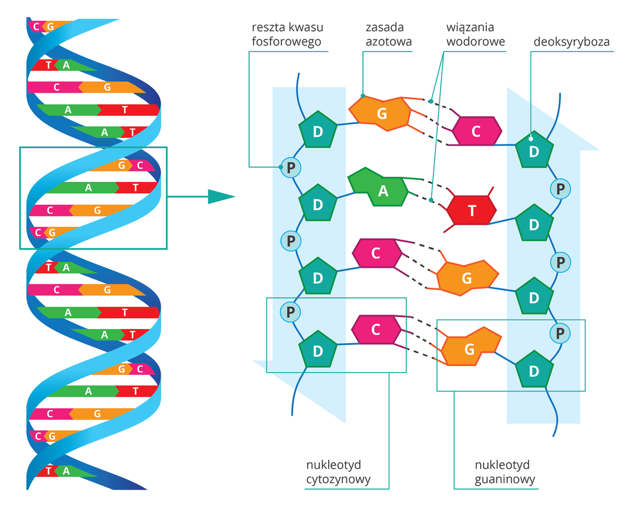
\includegraphics[width=0.5\textwidth]{dna1.png}
	\caption{Budowa podwójnej nici DNA.}
	\label{fig:}
\end{figure} \\
Przeprowadzenie sekwencjonowania DNA:
\begin{enumerate}
	\item \textbf{Powielanie badanego odcinka DNA.} \\
	Etap ten polega na wielokrotnej replikacji badanego odcinka DNA z użyciem zwykłych nukleotydów, które umożliwiają syntezę DNA, oraz znakowanych fluorescencyjnie nukleotydów, które po dołączeniu do nici natychmiast kończą syntezę DNA.
	W efekcie powstaje ogromna liczba kopii badanego odcinka DNA o różnej długości, zakończonych znakowanymi nukleotydami.
	\item \textbf{Ustalenie sekwencji DNA badanego odcinka.} \\
	W tym etapie kopie DNA są ustawiane w kolejności od najkrótszej do najdłuższej. Sekwenator rejestruje rodzaj emitowanego przez nie światła i na tej podstawie ustala sekwencję DNA.
	Ostatecznie otrzymujemy wydruk z ciągiem liter A, T, C i G, które oznaczają kolejne nukleotydy w DNA.
\end{enumerate}
\subsection{Technika PCR (łańcuchowa reakcja polimerazy)}%
\label{sub:Technika PCR (łańcuchowa reakcja polimerazy)}
Pozwala ona na uzyskanie w krótkim czasie dużej ilości kopii dowolnego fragmentu DNA. \texttt{Do dokończenia}
\subsection{Elektroforeza}%
\label{sub:Elektroforeza}
Jest to metoda, która umożliwia rozdzielenie fragmentów DNA w polu elektrycznym.
Elektroforezę wykorzystuje się m.in. do tworzenia profili genetyczych, czyli do ustalania długości określonych fragmentów DNA danej osoby.  \textbf{Przebieg elektroforezy DNA:} \begin{enumerate}
	\item Próbki DNA umieszcza się w odpowiednich miejscach na płytce i poddaje działaniu pola elektrycznego
	\item Pod wpływem pola elektrycznego ujemnie naładowane cząsteczki DNA przemieszczają się w kierunku bieguna dodatniego.
	\item Cząsteczki DNA poruszają się w żelu z różną prędkością i tworzą prążki. Krótsze fragmenty przemieszczają się zwykle szybciej.
\end{enumerate}
\section{Wykorzystanie technik inżynierii genetycznej w różnych dziedzinach.}%
\label{sec:Wykorzystanie technik inżynierii genetycznej w różnych dziedzinach.}
\textbf{W medycynie} wykorzystuje się m.in. do ustalania ojcostwa lub pokrewieństwa, np. w przypadku niektórych spraw spadkowych.
Pozwalają one także na indentyfikację zmarłych nawet po wielu latach od ich śmierci. \\
\textbf{W kryminalistyce}, na podstawie DNA pobranego z miejsca przestępstwa tworzy się profile genetyczne, dzięki którym można ustalić toższamość ofiar i sprawców przestępstw. (\textit{np. pozostawionego w odciskach palców.}) \\
\textbf{W diagnostyce chorób}, można ustalić sekwencje DNA pacjenta i określić, czy jest on nosicielem mutacji odpowiedzialnej za rozwój określonej choroby, lub wykryć materiał genetyczny patogenu powodującego chorobę.
\section{Czym są i jak uzyskuje się organizmy modyfikowane genetycznie (GMO)?}%
\label{sec:Czym są i jak uzyskuje się organizmy modyfikowane genetycznie (GMO)?}
\textbf{GMO} (\textit{ang. genetically modified organism}) to organizm, którego materiał genetyczny został zmieniony za pomocą technik inżynierii genetycznej. \\
Uzyskujemy GMO poprzez m.in:
\begin{itemize}
	\item \textbf{Zmianę aktywności w genomie} - oznacza to, że aktywuje się lub wycisza jeden z genów organizmu, co skutkuje obecnością lub brakiem wybranej cechy.
	\item \textbf{Zwielokrotnienie genu naturalnie występującego w genomie} - w efekcie w materiale genetycznym organizmu występują dodatkowe kopie jednego z jego genów.
	Powstaje wtedy większa ilość kodowanego przez ten gen białka.
	\item \textbf{Wprowadzenie do genomu organizmu genu pochodzącego od osobnika innego gatunku} - w konsekwencji organizm zaczyna produkować zupełnie nowe białko, dzięki czemu nabywa nową cechę.
	Organizm, który zawiera w swoim genomie obcy materiał genetyczny, nazywamy \textit{organizmem transgenicznym.}
\end{itemize}
\appendix
\section{Najważniejsze definicje}%
\label{sec:Najważniejsze definicje}

\tableofcontents
\end{document}
